\documentclass[]{article}
\usepackage{lmodern}
\usepackage{amssymb,amsmath}
\usepackage{ifxetex,ifluatex}
\usepackage{fixltx2e} % provides \textsubscript
\ifnum 0\ifxetex 1\fi\ifluatex 1\fi=0 % if pdftex
  \usepackage[T1]{fontenc}
  \usepackage[utf8]{inputenc}
\else % if luatex or xelatex
  \ifxetex
    \usepackage{mathspec}
  \else
    \usepackage{fontspec}
  \fi
  \defaultfontfeatures{Ligatures=TeX,Scale=MatchLowercase}
\fi
% use upquote if available, for straight quotes in verbatim environments
\IfFileExists{upquote.sty}{\usepackage{upquote}}{}
% use microtype if available
\IfFileExists{microtype.sty}{%
\usepackage{microtype}
\UseMicrotypeSet[protrusion]{basicmath} % disable protrusion for tt fonts
}{}
\usepackage[margin=1in]{geometry}
\usepackage{hyperref}
\hypersetup{unicode=true,
            pdftitle={Survival Analysis on the Primary Biliary Cirrhosis},
            pdfborder={0 0 0},
            breaklinks=true}
\urlstyle{same}  % don't use monospace font for urls
\usepackage{color}
\usepackage{fancyvrb}
\newcommand{\VerbBar}{|}
\newcommand{\VERB}{\Verb[commandchars=\\\{\}]}
\DefineVerbatimEnvironment{Highlighting}{Verbatim}{commandchars=\\\{\}}
% Add ',fontsize=\small' for more characters per line
\usepackage{framed}
\definecolor{shadecolor}{RGB}{248,248,248}
\newenvironment{Shaded}{\begin{snugshade}}{\end{snugshade}}
\newcommand{\KeywordTok}[1]{\textcolor[rgb]{0.13,0.29,0.53}{\textbf{#1}}}
\newcommand{\DataTypeTok}[1]{\textcolor[rgb]{0.13,0.29,0.53}{#1}}
\newcommand{\DecValTok}[1]{\textcolor[rgb]{0.00,0.00,0.81}{#1}}
\newcommand{\BaseNTok}[1]{\textcolor[rgb]{0.00,0.00,0.81}{#1}}
\newcommand{\FloatTok}[1]{\textcolor[rgb]{0.00,0.00,0.81}{#1}}
\newcommand{\ConstantTok}[1]{\textcolor[rgb]{0.00,0.00,0.00}{#1}}
\newcommand{\CharTok}[1]{\textcolor[rgb]{0.31,0.60,0.02}{#1}}
\newcommand{\SpecialCharTok}[1]{\textcolor[rgb]{0.00,0.00,0.00}{#1}}
\newcommand{\StringTok}[1]{\textcolor[rgb]{0.31,0.60,0.02}{#1}}
\newcommand{\VerbatimStringTok}[1]{\textcolor[rgb]{0.31,0.60,0.02}{#1}}
\newcommand{\SpecialStringTok}[1]{\textcolor[rgb]{0.31,0.60,0.02}{#1}}
\newcommand{\ImportTok}[1]{#1}
\newcommand{\CommentTok}[1]{\textcolor[rgb]{0.56,0.35,0.01}{\textit{#1}}}
\newcommand{\DocumentationTok}[1]{\textcolor[rgb]{0.56,0.35,0.01}{\textbf{\textit{#1}}}}
\newcommand{\AnnotationTok}[1]{\textcolor[rgb]{0.56,0.35,0.01}{\textbf{\textit{#1}}}}
\newcommand{\CommentVarTok}[1]{\textcolor[rgb]{0.56,0.35,0.01}{\textbf{\textit{#1}}}}
\newcommand{\OtherTok}[1]{\textcolor[rgb]{0.56,0.35,0.01}{#1}}
\newcommand{\FunctionTok}[1]{\textcolor[rgb]{0.00,0.00,0.00}{#1}}
\newcommand{\VariableTok}[1]{\textcolor[rgb]{0.00,0.00,0.00}{#1}}
\newcommand{\ControlFlowTok}[1]{\textcolor[rgb]{0.13,0.29,0.53}{\textbf{#1}}}
\newcommand{\OperatorTok}[1]{\textcolor[rgb]{0.81,0.36,0.00}{\textbf{#1}}}
\newcommand{\BuiltInTok}[1]{#1}
\newcommand{\ExtensionTok}[1]{#1}
\newcommand{\PreprocessorTok}[1]{\textcolor[rgb]{0.56,0.35,0.01}{\textit{#1}}}
\newcommand{\AttributeTok}[1]{\textcolor[rgb]{0.77,0.63,0.00}{#1}}
\newcommand{\RegionMarkerTok}[1]{#1}
\newcommand{\InformationTok}[1]{\textcolor[rgb]{0.56,0.35,0.01}{\textbf{\textit{#1}}}}
\newcommand{\WarningTok}[1]{\textcolor[rgb]{0.56,0.35,0.01}{\textbf{\textit{#1}}}}
\newcommand{\AlertTok}[1]{\textcolor[rgb]{0.94,0.16,0.16}{#1}}
\newcommand{\ErrorTok}[1]{\textcolor[rgb]{0.64,0.00,0.00}{\textbf{#1}}}
\newcommand{\NormalTok}[1]{#1}
\usepackage{graphicx,grffile}
\makeatletter
\def\maxwidth{\ifdim\Gin@nat@width>\linewidth\linewidth\else\Gin@nat@width\fi}
\def\maxheight{\ifdim\Gin@nat@height>\textheight\textheight\else\Gin@nat@height\fi}
\makeatother
% Scale images if necessary, so that they will not overflow the page
% margins by default, and it is still possible to overwrite the defaults
% using explicit options in \includegraphics[width, height, ...]{}
\setkeys{Gin}{width=\maxwidth,height=\maxheight,keepaspectratio}
\IfFileExists{parskip.sty}{%
\usepackage{parskip}
}{% else
\setlength{\parindent}{0pt}
\setlength{\parskip}{6pt plus 2pt minus 1pt}
}
\setlength{\emergencystretch}{3em}  % prevent overfull lines
\providecommand{\tightlist}{%
  \setlength{\itemsep}{0pt}\setlength{\parskip}{0pt}}
\setcounter{secnumdepth}{5}
% Redefines (sub)paragraphs to behave more like sections
\ifx\paragraph\undefined\else
\let\oldparagraph\paragraph
\renewcommand{\paragraph}[1]{\oldparagraph{#1}\mbox{}}
\fi
\ifx\subparagraph\undefined\else
\let\oldsubparagraph\subparagraph
\renewcommand{\subparagraph}[1]{\oldsubparagraph{#1}\mbox{}}
\fi

%%% Use protect on footnotes to avoid problems with footnotes in titles
\let\rmarkdownfootnote\footnote%
\def\footnote{\protect\rmarkdownfootnote}

%%% Change title format to be more compact
\usepackage{titling}

% Create subtitle command for use in maketitle
\newcommand{\subtitle}[1]{
  \posttitle{
    \begin{center}\large#1\end{center}
    }
}

\setlength{\droptitle}{-2em}

  \title{Survival Analysis on the Primary Biliary Cirrhosis}
    \pretitle{\vspace{\droptitle}\centering\huge}
  \posttitle{\par}
    \author{}
    \preauthor{}\postauthor{}
      \predate{\centering\large\emph}
  \postdate{\par}
    \date{November 2018}


\begin{document}
\maketitle

{
\setcounter{tocdepth}{2}
\tableofcontents
}
\section{Introduction}\label{introduction}

Multiple tools and data for survival analysis are available in R
packages such as ``survival'' from where we picked the PBC dataset. It
comes from a clinical trial in the field of primary biliary cirrhosis
conducted at the Mayo Clinic between 1974 and 1984. Primary biliary
cirrhosis is a fatal chronic liver disease.

A total of 418 PBC patients were randomized to either a placebo or a
drug called D-penicillamine. Each of them was followed until death or
censoring (the duration is measured in days). The status at endpoint is
coded as follows: 0/1/2 for censored, transplant and dead respectively.
In addition, 17 covariates are recorded for this study. These include a
treatment variable, patient age, gender and clinical, biochemical and
histologic measurements made at the time of randomization.

After preparing the data for in depth survival analysis (in part 2), the
present work aimed to answer various questions related to the survival
of the studied patients with biliary cirrhosis. From the very first one
being ``What does the survival of the patients look like overall?'' we
explicitely confronted their survival to selected covariates (part 3.3).
We then studied the potentially existing differences between groups
through unique covariates (part 3.4) and assessed both isolated and
joint impact of progressively selected covariates on the survival
through statistical significance (part 3.5). We finally produced the
tests diagnostics (part 3.6) and concluded.

\section{Data preparation}\label{data-preparation}

\subsection{Libraries importation}\label{libraries-importation}

We also ground the present document on various other packages for model
elaboration (ie. glmnet, survival) and data presentation (ie. gglopt2,
readr, glmnet \ldots{}etc.).

\begin{Shaded}
\begin{Highlighting}[]
\KeywordTok{library}\NormalTok{(ggplot2)}
\KeywordTok{library}\NormalTok{(survminer)}
\end{Highlighting}
\end{Shaded}

\begin{verbatim}
## Loading required package: ggpubr
\end{verbatim}

\begin{verbatim}
## Loading required package: magrittr
\end{verbatim}

\begin{Shaded}
\begin{Highlighting}[]
\KeywordTok{library}\NormalTok{(readr)}
\KeywordTok{library}\NormalTok{(glmnet)}
\end{Highlighting}
\end{Shaded}

\begin{verbatim}
## Loading required package: Matrix
\end{verbatim}

\begin{verbatim}
## Loading required package: foreach
\end{verbatim}

\begin{verbatim}
## Loaded glmnet 2.0-16
\end{verbatim}

\begin{Shaded}
\begin{Highlighting}[]
\KeywordTok{library}\NormalTok{(survival)}
\end{Highlighting}
\end{Shaded}

\subsection{\texorpdfstring{Specify event as status ==
``death''}{Specify event as status == death}}\label{specify-event-as-status-death}

Declare data importation and event association to the death of the
patient corresponding to the status parameter returning ``2''.
Transplantation cases (status parameter returning ``1'') were not
considered in the context of a survival analysis, stricto sensu.

\begin{Shaded}
\begin{Highlighting}[]
\CommentTok{# assign data set to a labelled object}
\NormalTok{data <-}\StringTok{ }\NormalTok{pbc}
\CommentTok{# create event parameter corresponding to death of the patient}
\NormalTok{data}\OperatorTok{$}\NormalTok{event <-}\StringTok{ }\DecValTok{0} \OperatorTok{+}\StringTok{ }\NormalTok{(data}\OperatorTok{$}\NormalTok{status }\OperatorTok{==}\StringTok{ }\DecValTok{2}\NormalTok{)}
\end{Highlighting}
\end{Shaded}

\subsection{Convert the necessary covariates into
factor}\label{convert-the-necessary-covariates-into-factor}

\begin{Shaded}
\begin{Highlighting}[]
\NormalTok{data}\OperatorTok{$}\NormalTok{trt <-}\StringTok{ }\KeywordTok{factor}\NormalTok{(data}\OperatorTok{$}\NormalTok{trt)}
\NormalTok{data}\OperatorTok{$}\NormalTok{status <-}\StringTok{ }\KeywordTok{factor}\NormalTok{(data}\OperatorTok{$}\NormalTok{status)}
\NormalTok{data}\OperatorTok{$}\NormalTok{stage <-}\StringTok{ }\KeywordTok{factor}\NormalTok{(data}\OperatorTok{$}\NormalTok{stage)}
\NormalTok{data}\OperatorTok{$}\NormalTok{ascites <-}\StringTok{ }\KeywordTok{factor}\NormalTok{(data}\OperatorTok{$}\NormalTok{ascites)}
\NormalTok{data}\OperatorTok{$}\NormalTok{edema <-}\StringTok{ }\KeywordTok{factor}\NormalTok{(data}\OperatorTok{$}\NormalTok{edema)}
\NormalTok{data}\OperatorTok{$}\NormalTok{spiders <-}\StringTok{ }\KeywordTok{factor}\NormalTok{(data}\OperatorTok{$}\NormalTok{spiders)}
\NormalTok{data}\OperatorTok{$}\NormalTok{hepato <-}\StringTok{ }\KeywordTok{factor}\NormalTok{(data}\OperatorTok{$}\NormalTok{hepato)}
\end{Highlighting}
\end{Shaded}

\subsection{Create age intervals}\label{create-age-intervals}

Printing the histogram of the age variable helped naively identifying
gaps or cuts in its distribution. This would highlight the number of
modes encompassed in the variable. Obvious gaps would suggest cutoffs on
which basing the creation of age groups variable.

\begin{Shaded}
\begin{Highlighting}[]
\KeywordTok{hist}\NormalTok{(data}\OperatorTok{$}\NormalTok{age, }\DataTypeTok{xlab=}\StringTok{"Age"}\NormalTok{)}
\end{Highlighting}
\end{Shaded}

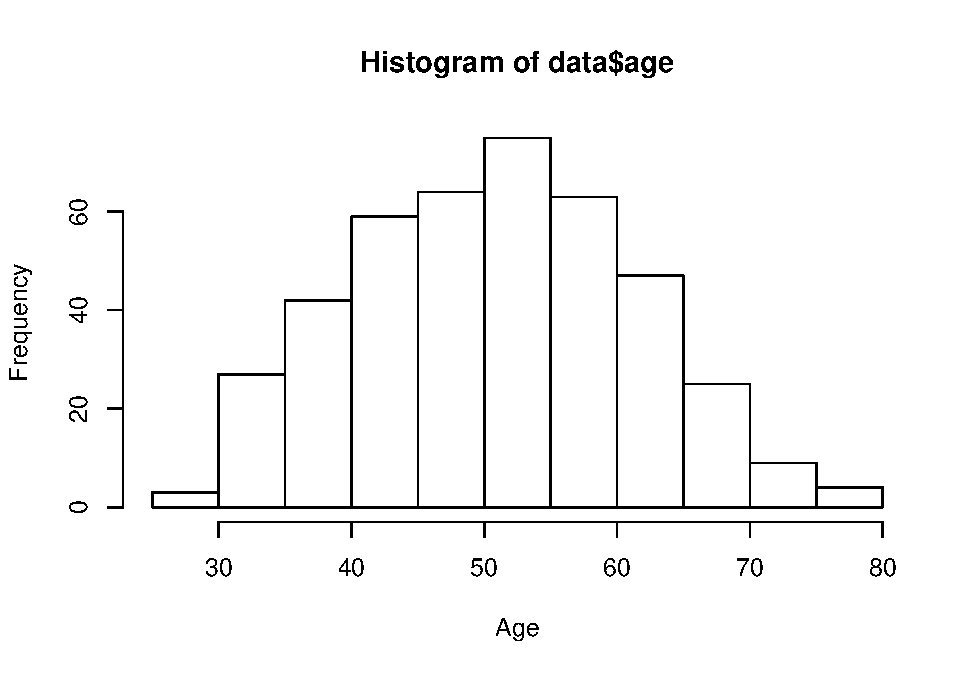
\includegraphics{report_files/figure-latex/unnamed-chunk-4-1.pdf}

As the output shown, we observed a ``properly'' distributed age variable
with no cuts or gaps thus implying an ageGroup variable ``evenly''"
distributed too.

\begin{Shaded}
\begin{Highlighting}[]
\NormalTok{data}\OperatorTok{$}\NormalTok{ageGroup <-}\StringTok{ }\KeywordTok{cut}\NormalTok{(data}\OperatorTok{$}\NormalTok{age, }\DataTypeTok{breaks =} \KeywordTok{c}\NormalTok{(}\DecValTok{0}\NormalTok{,}\DecValTok{10}\NormalTok{,}\DecValTok{20}\NormalTok{,}\DecValTok{30}\NormalTok{,}\DecValTok{40}\NormalTok{,}\DecValTok{50}\NormalTok{,}\DecValTok{60}\NormalTok{,}\DecValTok{70}\NormalTok{,}\DecValTok{80}\NormalTok{,}\DecValTok{90}\NormalTok{,}\OtherTok{Inf}\NormalTok{))}
\KeywordTok{table}\NormalTok{(data}\OperatorTok{$}\NormalTok{ageGroup)}
\end{Highlighting}
\end{Shaded}

\begin{verbatim}
## 
##   (0,10]  (10,20]  (20,30]  (30,40]  (40,50]  (50,60]  (60,70]  (70,80] 
##        0        0        3       69      123      138       72       13 
##  (80,90] (90,Inf] 
##        0        0
\end{verbatim}

\subsection{Input some missing values}\label{input-some-missing-values}

Few observable missing values required us to apply linear model
predictions in order to be refined. The reader might be interested in an
example line of code as displayed below:

\begin{Shaded}
\begin{Highlighting}[]
\CommentTok{# for chol (cholesterol) parameter }
\NormalTok{fit.chol <-}\StringTok{ }\NormalTok{(}\KeywordTok{lm}\NormalTok{(chol }\OperatorTok{~}\StringTok{ }\NormalTok{age, }\DataTypeTok{data =}\NormalTok{ data))}
\NormalTok{data}\OperatorTok{$}\NormalTok{chol[}\KeywordTok{is.na}\NormalTok{(data}\OperatorTok{$}\NormalTok{chol)] <-}
\StringTok{  }\KeywordTok{predict}\NormalTok{(fit.chol, }\DataTypeTok{newdata =} \KeywordTok{subset}\NormalTok{(data, }\KeywordTok{is.na}\NormalTok{(chol)))}
\end{Highlighting}
\end{Shaded}

Raw data having been treated at this point, we could enter the
exploratory analysis phase of the data set.

\section{Exploratory analysis}\label{exploratory-analysis}

It started with the creation of the data subset to be studied according
the following rule.

\subsection{Locate patients for survival
analysis}\label{locate-patients-for-survival-analysis}

Our patient's type-profile encompassed : - patients that followed a
treatment, thus excluding the 106 patients that did not; - patients
concerned by the event of their death or consored, thus excluding the
patients that were transplanted.

\begin{Shaded}
\begin{Highlighting}[]
\NormalTok{specimen <-}\StringTok{ }\KeywordTok{subset}\NormalTok{(data, data}\OperatorTok{$}\NormalTok{trt }\OperatorTok{!=}\StringTok{ "NA"} \OperatorTok{&}\StringTok{ }\NormalTok{data}\OperatorTok{$}\NormalTok{status }\OperatorTok{!=}\StringTok{ }\DecValTok{1}\NormalTok{)}
\KeywordTok{summary}\NormalTok{(specimen)}
\end{Highlighting}
\end{Shaded}

\begin{verbatim}
##        id             time      status  trt          age        sex    
##  Min.   :  1.0   Min.   :  41   0:168   1:148   Min.   :26.28   m: 33  
##  1st Qu.: 75.0   1st Qu.:1216   1:  0   2:145   1st Qu.:42.97   f:260  
##  Median :152.0   Median :1882   2:125           Median :50.54          
##  Mean   :152.9   Mean   :2039                   Mean   :50.59          
##  3rd Qu.:227.0   3rd Qu.:2772                   3rd Qu.:57.20          
##  Max.   :312.0   Max.   :4556                   Max.   :78.44          
##                                                                        
##  ascites hepato  spiders edema          bili             chol       
##  0:269   0:145   0:208   0  :246   Min.   : 0.300   Min.   : 120.0  
##  1: 24   1:148   1: 85   0.5: 27   1st Qu.: 0.800   1st Qu.: 253.0  
##                          1  : 20   Median : 1.300   Median : 316.0  
##                                    Mean   : 3.264   Mean   : 365.0  
##                                    3rd Qu.: 3.400   3rd Qu.: 397.9  
##                                    Max.   :28.000   Max.   :1775.0  
##                                                                     
##     albumin          copper          alk.phos          ast        
##  Min.   :1.960   Min.   :  4.00   Min.   :  289   Min.   : 26.35  
##  1st Qu.:3.310   1st Qu.: 41.00   1st Qu.:  858   1st Qu.: 79.05  
##  Median :3.550   Median : 70.00   Median : 1258   Median :111.00  
##  Mean   :3.517   Mean   : 95.93   Mean   : 2012   Mean   :122.07  
##  3rd Qu.:3.800   3rd Qu.:123.00   3rd Qu.: 2009   3rd Qu.:151.90  
##  Max.   :4.640   Max.   :588.00   Max.   :13862   Max.   :457.25  
##                  NA's   :2                                        
##       trig           platelet        protime      stage       event       
##  Min.   : 44.00   Min.   : 62.0   Min.   : 9.00   1: 16   Min.   :0.0000  
##  1st Qu.: 84.75   1st Qu.:195.0   1st Qu.:10.00   2: 64   1st Qu.:0.0000  
##  Median :108.00   Median :253.0   Median :10.60   3:112   Median :0.0000  
##  Mean   :124.07   Mean   :259.5   Mean   :10.75   4:101   Mean   :0.4266  
##  3rd Qu.:151.25   3rd Qu.:322.0   3rd Qu.:11.10           3rd Qu.:1.0000  
##  Max.   :598.00   Max.   :563.0   Max.   :17.10           Max.   :1.0000  
##  NA's   :29       NA's   :4                                               
##     ageGroup 
##  (50,60]:96  
##  (40,50]:90  
##  (30,40]:47  
##  (60,70]:46  
##  (70,80]:11  
##  (20,30]: 3  
##  (Other): 0
\end{verbatim}

Getting a 293 observations data set on, called ``specimen'', which we
now would be able to run the survival analysis related tests as below.

\subsection{Create survival objects}\label{create-survival-objects}

Survival objects are created through the Surv(time, status) function
from the ``survival'' package. To create right-censored data, this
function needs two arguments: - time: returns the observed duration in
days; - status: returns a boolean regarding whereas the observation
corresponds to a censored one or not.

In the situation where status returns more than two modalities or if the
modalities are not returning a boolean, conditioned by the fact that the
observations are censored or not, the formula creating the survival
object must precise the proper modalities corresponding to censored
observations.

\begin{Shaded}
\begin{Highlighting}[]
\NormalTok{survival <-}\StringTok{ }\KeywordTok{Surv}\NormalTok{(specimen}\OperatorTok{$}\NormalTok{time }\OperatorTok{/}\StringTok{ }\FloatTok{365.25}\NormalTok{, specimen}\OperatorTok{$}\NormalTok{event)}
\end{Highlighting}
\end{Shaded}

Hereby computed with time alteration to show yearly-basis scale for
lisibility purpose of the reader.

\subsection{Kaplan-Meyer estimator - estimation of the survival
function}\label{kaplan-meyer-estimator---estimation-of-the-survival-function}

Also known as ``product-limit estimator'', the Kaplan-Meyer estimator
(KM) is a non-parametric statistic (ie. not based on the assumption of
an underlying probability distribution) that allows one to estimate the
survival function. It gives the probability that an individual patient
will survive past a particular time ``t''. It is based on the assumption
that the probability of surviving past this point is equal to the
product of the observed survival rates until time point ``t''. It is
similar to the censoring version of empirical survival function,
generating a stair-step curve but not accounting for effect of other
covariates.

Applying the Kaplan-Meyer estimator helped answer the question ``How is
the survival of the overall studied sample shaped like?''

In R, the estimation of a survival function through the use of a
survival object (ie. from censored data) is done thanks to the
survfit(Surv(time, status), data) function of the ``survival'' package.

\begin{Shaded}
\begin{Highlighting}[]
\NormalTok{KM <-}\StringTok{ }\KeywordTok{survfit}\NormalTok{(survival }\OperatorTok{~}\StringTok{ }\DecValTok{1}\NormalTok{, }\DataTypeTok{data =}\NormalTok{ specimen)}
\NormalTok{KM}
\end{Highlighting}
\end{Shaded}

\begin{verbatim}
## Call: survfit(formula = survival ~ 1, data = specimen)
## 
##       n  events  median 0.95LCL 0.95UCL 
##  293.00  125.00    8.99    7.79   10.51
\end{verbatim}

\begin{Shaded}
\begin{Highlighting}[]
\KeywordTok{ggsurvplot}\NormalTok{(KM, }\DataTypeTok{xlab=}\StringTok{"Survival Years"}\NormalTok{, }\DataTypeTok{ylab=}\StringTok{"Kaplan-Meyer Estimator"}\NormalTok{)}
\end{Highlighting}
\end{Shaded}

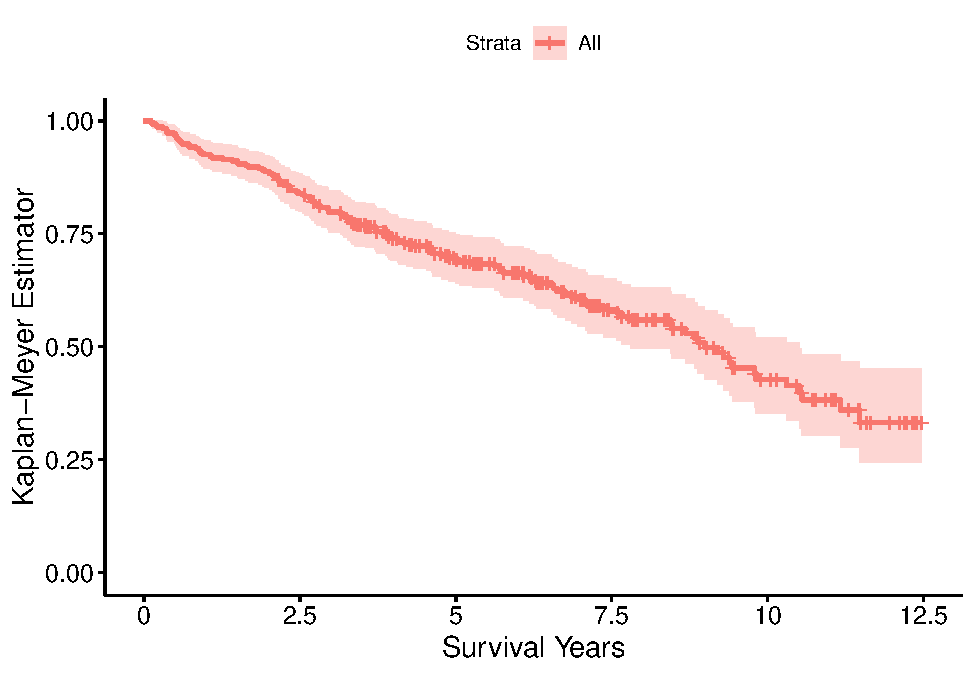
\includegraphics{report_files/figure-latex/unnamed-chunk-9-1.pdf}

The KM test returned a median survival of 8.99 years, the moment at
which 50\% of the patients were alive and 50\% were reaching the event
point ie. here, death. On a broader note, the reader may be interested
in visualizing the survival regarding other parameters. This have been
realised by crossing the survival object with the specific parameters
through additional KM tests as shown below.

One might state that interesting parameters to be confronted to survival
are sex, trt (for treatment parameter) and age, the later requiring a
preparation to its study (ie. ``binarizing'' the sample into ``younger''
vs ``older'' patients for example).

First trying to answer the question: ``How is the overall survival
shaped like regarding patients gender?''

\begin{Shaded}
\begin{Highlighting}[]
\CommentTok{# fitting the survival to sex parameter}
\NormalTok{fit.sex <-}\StringTok{ }\KeywordTok{survfit}\NormalTok{(survival }\OperatorTok{~}\StringTok{ }\NormalTok{sex, }\DataTypeTok{data =}\NormalTok{ specimen)}
\NormalTok{## visualizing the survival probability}
\KeywordTok{ggsurvplot}\NormalTok{(fit.sex, }
           \DataTypeTok{data =}\NormalTok{ specimen, }
           \DataTypeTok{xlab =} \StringTok{"Years"}\NormalTok{,}
           \DataTypeTok{conf.int =} \OtherTok{FALSE}\NormalTok{,}
           \DataTypeTok{pval =} \OtherTok{TRUE}\NormalTok{,}
           \DataTypeTok{legend =} \StringTok{"top"}\NormalTok{,}
           \DataTypeTok{legend.title =} \StringTok{"Sex"}\NormalTok{,}
           \DataTypeTok{legend.labs =} \KeywordTok{c}\NormalTok{(}\StringTok{"Male"}\NormalTok{, }\StringTok{"Female"}\NormalTok{))}
\end{Highlighting}
\end{Shaded}

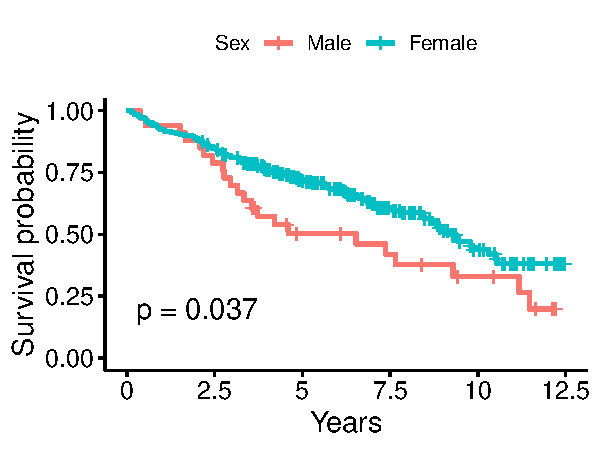
\includegraphics{report_files/figure-latex/unnamed-chunk-10-1.pdf}

Additionally to the general shape of the curves, the reader might be
interested in the p-value shown at the bottom-left of the figure which
is the corresponding log-rank test p-value result. Here statistically
significant, as under an arbitrary threshold of 5\% (corresponding to a
95\% confidence interval) it conveys enough significance to reject the
log-rank null hypothesis and affirm that the two groups, here male \&
female, survive differently to the biliary cirrhosis.

Explicitly, the output above shown that men have a worse survival
expectancy than women to biliary cirrhosis. The reader might be
interested in noting that the number of censored data for female
patients appear to be greater than the ones of male patients, one might
naively state that it would be concuring the above results.

Now considering the treatment parameter (D-penicillamin vs.~placebo),
thus answering the question: ``How is the overall survival shaped like
regarding patients administred treatment?''

\begin{Shaded}
\begin{Highlighting}[]
\CommentTok{# fitting the survival to treatment parameter}
\NormalTok{fit.trt <-}\StringTok{ }\KeywordTok{survfit}\NormalTok{(survival }\OperatorTok{~}\StringTok{ }\NormalTok{trt, }\DataTypeTok{data =}\NormalTok{ specimen)}
\NormalTok{## visualizing the survival probability}
\KeywordTok{ggsurvplot}\NormalTok{(fit.trt, }
           \DataTypeTok{data =}\NormalTok{ specimen, }
           \DataTypeTok{xlab =} \StringTok{"Years"}\NormalTok{,}
           \DataTypeTok{conf.int =} \OtherTok{FALSE}\NormalTok{,}
           \DataTypeTok{pval =} \OtherTok{TRUE}\NormalTok{,}
           \DataTypeTok{legend =} \StringTok{"top"}\NormalTok{,}
           \DataTypeTok{legend.title =} \StringTok{"Treatment"}\NormalTok{,}
           \DataTypeTok{legend.labs =} \KeywordTok{c}\NormalTok{(}\StringTok{"D-penicillamin"}\NormalTok{, }\StringTok{"Placebo"}\NormalTok{))}
\end{Highlighting}
\end{Shaded}

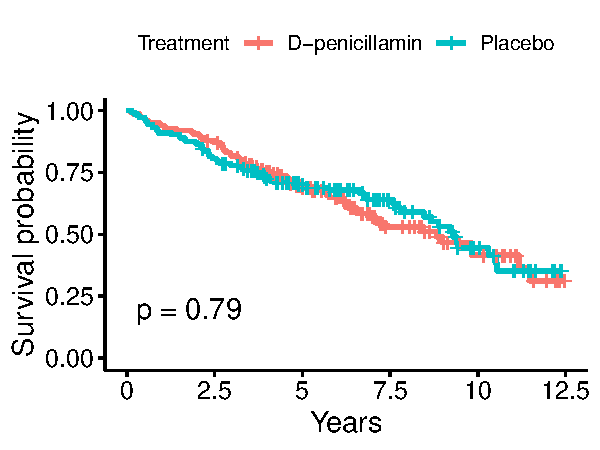
\includegraphics{report_files/figure-latex/unnamed-chunk-11-1.pdf}

As the reader might visually build an intuition of the difference in
treatment parameter, the resulting non-significant p-value (79\%)
indicates that there is not enough statistical material in order to
reject the null hypothesis and thus leads one to conclude that there is
no significant difference between both treatment protocols. Explicitly,
whereas taking a D-penicillamin treatment or a placebo treatment has no
impact on patients survival expectancy.

Finally one may think an additional useful visualization to the reader
would be the study of the survival object regarding the age parameter.
As stated earlier it appeared necessary to retreat the age parameter in
order to make it senseful to the KM and log-rank tests by ``binarizing''
it as shown in the following, aiming to answer the question: ``How is
the overall survival shaped like regarding patients relative age?''

\begin{Shaded}
\begin{Highlighting}[]
\CommentTok{# age parameter retreatment named "ageBin" parameter}
\NormalTok{specimen}\OperatorTok{$}\NormalTok{ageBin <-}\StringTok{ }\KeywordTok{ifelse}\NormalTok{(specimen}\OperatorTok{$}\NormalTok{age }\OperatorTok{>}\StringTok{ }\DecValTok{50}\NormalTok{, }\StringTok{">50"}\NormalTok{, }\StringTok{"<=50"}\NormalTok{)}
\CommentTok{# converting the ageBin parameter into factor}
\NormalTok{specimen}\OperatorTok{$}\NormalTok{ageBin <-}\StringTok{ }\KeywordTok{as.factor}\NormalTok{(specimen}\OperatorTok{$}\NormalTok{ageBin)}
\CommentTok{# fitting the survival to the new age parameter}
\NormalTok{fit.age <-}\StringTok{ }\KeywordTok{survfit}\NormalTok{(survival }\OperatorTok{~}\StringTok{ }\NormalTok{ageBin, }\DataTypeTok{data =}\NormalTok{ specimen)}
\NormalTok{## visualizing the survival probability}
\KeywordTok{ggsurvplot}\NormalTok{(fit.age, }
           \DataTypeTok{data =}\NormalTok{ specimen, }
           \DataTypeTok{xlab =} \StringTok{"Years"}\NormalTok{,}
           \DataTypeTok{conf.int =} \OtherTok{FALSE}\NormalTok{,}
           \DataTypeTok{pval =} \OtherTok{TRUE}\NormalTok{,}
           \DataTypeTok{legend =} \StringTok{"top"}\NormalTok{,}
           \DataTypeTok{legend.title =} \StringTok{"Age"}\NormalTok{,}
           \DataTypeTok{legend.labs =} \KeywordTok{c}\NormalTok{(}\StringTok{"Youngers (<=50)"}\NormalTok{, }\StringTok{"Olders (>50)"}\NormalTok{))}
\end{Highlighting}
\end{Shaded}

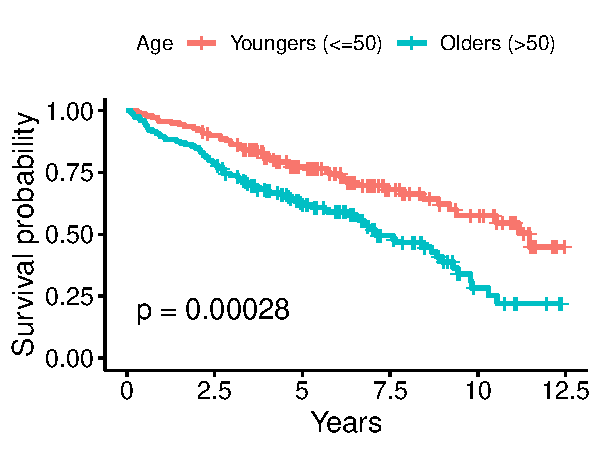
\includegraphics{report_files/figure-latex/unnamed-chunk-12-1.pdf}

Here again as the reader may have an intuition of the potential
difference in survival regarding the age parameter as shown by the
shapes of the curves, the resulting p-value (0.028\%) indicates that
there exists a statistically significant difference in the survival of
the two groups segmented through the age parameter. Explicitly the
``olders'', the patients who's age is greater than fifty years old, have
a worse survival expectancy over time than the ``youngers'', the
patients who's age is lower or equal to fifty years old.

The provided p-value to the KM visualization of the survival object
introduced the reader to the observation of differences in some
parameters variable to be explicited in the Mantel-Haenzel test, also
called the log-rank test.

\subsection{Mantel-Haenzel test - comparing two groups' own
survival}\label{mantel-haenzel-test---comparing-two-groups-own-survival}

Also known as log-rank test, it is a statistical hypothesis test that
tests the null hypothesis that survival curves of two populations do not
differ. It will output an indicator of the two groups being
significantly different in terms of survival when its p-value will be
inferior to risk threshold.

It is efficient in comparing groups differed by categorical variables,
but not continuous ones. Its validity conditions might appear quite
delicate to the reader as the log-rank test, to be considered as
applicable, requires or an important number of death times which mathcs
the situation of our sample study, or an important number of deads at
each death time.

Nonetheless it appeared necessary to answer the question: ``Is survival
different for patients who were administred one treatment rather than
the other?''

\begin{Shaded}
\begin{Highlighting}[]
\NormalTok{MH <-}\StringTok{ }\KeywordTok{survdiff}\NormalTok{(survival }\OperatorTok{~}\StringTok{ }\NormalTok{specimen}\OperatorTok{$}\NormalTok{trt)}
\NormalTok{MH}
\end{Highlighting}
\end{Shaded}

\begin{verbatim}
## Call:
## survdiff(formula = survival ~ specimen$trt)
## 
##                  N Observed Expected (O-E)^2/E (O-E)^2/V
## specimen$trt=1 148       65     63.5    0.0354    0.0722
## specimen$trt=2 145       60     61.5    0.0366    0.0722
## 
##  Chisq= 0.1  on 1 degrees of freedom, p= 0.8
\end{verbatim}

The log-rank test returned a non-significant p-value (80\%) indicating
that one does not have enough elements to reject the null hypothesis
allowing to interprete that there is no statistically significant
difference between the two treatments. Concurring the earlier
interpretation, whereas a patient was administered D-penicillamin or
placebo had no impact on the patient's survival expectancy.

An alternative test, the Wilcoxon test may be applied in order to
compare the significance of the result with the one from the log-rank
test. However the reader will be advised that : \emph{the log-rank test
is more effective when the survival curves do not cross each other;
}when instantaneous hazard rates are proportional, the log-rank test is
the ``best'' to be run.

\begin{Shaded}
\begin{Highlighting}[]
\NormalTok{W <-}\StringTok{ }\KeywordTok{survdiff}\NormalTok{(survival }\OperatorTok{~}\StringTok{ }\NormalTok{specimen}\OperatorTok{$}\NormalTok{trt, }\DataTypeTok{rho=}\DecValTok{1}\NormalTok{)}
\NormalTok{W}
\end{Highlighting}
\end{Shaded}

\begin{verbatim}
## Call:
## survdiff(formula = survival ~ specimen$trt, rho = 1)
## 
##                  N Observed Expected (O-E)^2/E (O-E)^2/V
## specimen$trt=1 148     49.1     48.7   0.00370   0.00949
## specimen$trt=2 145     46.3     46.7   0.00385   0.00949
## 
##  Chisq= 0  on 1 degrees of freedom, p= 0.9
\end{verbatim}

Having returned a greater p-value for the log-rank test, it prevented
from rejecting the null hypothesis, concurring the earlier
interpretation, leading to conclude that there is no statistically
significant difference between the two studied groups ie. whereas
patients were administred D-penicillamin or placebo.

Various groups having been studied and compared regarding different
perspectives, another complementary approach would be association of
survival to a quantitative variable, allowed by the Cox model as
presented in the following part.

\subsection{Cox Model Regressions}\label{cox-model-regressions}

Also known as proportional hazard model, it conveniently accesses the
effect of continuous and categorical variable using partial likelihood
to get inference even without knowledge of baseline hazard.

While the log-rank test compares two Kaplan-Meier survival curves, which
might be derived from splitting a patient population into treatment
subgroups, Cox proportional hazards model regressions are derived from
the underlying baseline hazard functions of the specific patient
populations studied and an arbitrary number of dichotomized covariates.
Again, it does not assume an underlying probability distribution but it
does assume that the hazards of the compared patient groupsare constant
over time.

The reader be advised that the presented approach was first to process
univariate Cox regressions fitting the three covariates : sex, treatment
\& age. This would supposedly help answering the question ``Do
specifically selected covariates (sex, treatment \& age) independently
and significantly impact survival and how?''

The second step of the approach has been to process a multivariate Cox
regression on all the covariates of the sample in order to identify the
most significant ones on patients survival expectancy and then return a
multivariate Cox regression on the selected covariates. This would help
us answer the question ``Which of covariates from the data set jointly
and significantly impact survival and how?''

First then, one may want to describe if and how the sex, treatment \&
age parameters independently impact on survival:

\begin{Shaded}
\begin{Highlighting}[]
\CommentTok{# univariate cox regression on sex parameter}
\NormalTok{cox.sex <-}\StringTok{ }\KeywordTok{coxph}\NormalTok{(survival }\OperatorTok{~}\StringTok{ }\NormalTok{sex, }\DataTypeTok{data =}\NormalTok{ specimen)}
\NormalTok{cox.sex}
\end{Highlighting}
\end{Shaded}

\begin{verbatim}
## Call:
## coxph(formula = survival ~ sex, data = specimen)
## 
##         coef exp(coef) se(coef)     z      p
## sexf -0.4872    0.6143   0.2365 -2.06 0.0394
## 
## Likelihood ratio test=3.82  on 1 df, p=0.05064
## n= 293, number of events= 125
\end{verbatim}

\begin{Shaded}
\begin{Highlighting}[]
\CommentTok{# univariate cox regression on treatment parameter}
\NormalTok{cox.trt <-}\StringTok{ }\KeywordTok{coxph}\NormalTok{(survival }\OperatorTok{~}\StringTok{ }\NormalTok{trt, }\DataTypeTok{data =}\NormalTok{ specimen)}
\NormalTok{cox.trt}
\end{Highlighting}
\end{Shaded}

\begin{verbatim}
## Call:
## coxph(formula = survival ~ trt, data = specimen)
## 
##          coef exp(coef) se(coef)      z     p
## trt2 -0.04823   0.95292  0.17917 -0.269 0.788
## 
## Likelihood ratio test=0.07  on 1 df, p=0.7877
## n= 293, number of events= 125
\end{verbatim}

\begin{Shaded}
\begin{Highlighting}[]
\CommentTok{# univariate cox regression on age parameter}
\NormalTok{cox.age <-}\StringTok{ }\KeywordTok{coxph}\NormalTok{(survival }\OperatorTok{~}\StringTok{ }\NormalTok{age, }\DataTypeTok{data =}\NormalTok{ specimen)}
\NormalTok{cox.age}
\end{Highlighting}
\end{Shaded}

\begin{verbatim}
## Call:
## coxph(formula = survival ~ age, data = specimen)
## 
##         coef exp(coef) se(coef)     z        p
## age 0.036526  1.037201 0.008903 4.103 4.08e-05
## 
## Likelihood ratio test=16.81  on 1 df, p=4.13e-05
## n= 293, number of events= 125
\end{verbatim}

The reader may be interested in the description of the numerous
interpretable outputs provided by the Cox Model regressions for the sake
of clarity : First, the ``input p-value'' indicates whereas there is a
statistically significant association between a given variable and the
hazard (risk of the event, here death). The statistical significance
marked by the ``z'' column assessing whether the beta coefficient of a
given variable is statistically significantly different from 0 by
measuring each regression coefficient to its standard error. The sign of
the regression coefficient with a positive (negative) sign implying a
higher (lower) hazard, with the specificity for variables encoded as
numeric vectors, here as for sex parameter (1=male, 2=female) and
treatment parameter (1=D-penicillamin, 2=placebo), that the coefficient
assesses the second group relative to the first one. The hazard ratio
giving the effect size of covariates. The global statistical
significance of the model is brought by the ``output p-value'' given for
overall significance of the model, the likelihood-ratio test.

Now from the output above, one would carrefully interprete the results
by stating that : \emph{both sex \& age parameters have a statistically
significant association with the hazard of the patients produced by
biliary cirrhosis (ie. p-value of 3.9\% \& c.0\% respectively) }both sex
\& age parameters have highly statistically significant coefficients
\emph{on one hand a beta of -0.49 indicates that females have lower risk
of death than males and that on another hand older patients have a
higher risk of death regarding biliary cirrhosis }being a female patient
reduces the hazard by a factor of 0.61 or 39\% thus associated with a
relatively better prognostic. Besides, one can estimate that a 3.7\%
greater risk of death is associated with a 1-year increase in age at
diagnosis *the p-value being associated to c.0\%, the model is indeed
significant

With these elements in mind, one may now want to describe how the
factors jointly impact on survival. Answering this question required
performing a multivariate Cox regression analysis. As the treatment
parameter was not significant in the univariate Cox analysis, it was
omitted from the multivariate analysis.

\begin{Shaded}
\begin{Highlighting}[]
\CommentTok{# multivariate cox regression}
\NormalTok{coxph <-}\StringTok{ }\KeywordTok{coxph}\NormalTok{(survival  }\OperatorTok{~}\StringTok{ }\NormalTok{age }\OperatorTok{+}\StringTok{ }\NormalTok{edema }\OperatorTok{+}\StringTok{ }\NormalTok{hepato }\OperatorTok{+}\StringTok{ }\NormalTok{platelet }\OperatorTok{+}\StringTok{ }\NormalTok{sex }\OperatorTok{+}\StringTok{ }\NormalTok{spiders }\OperatorTok{+}\StringTok{ }\NormalTok{ascites }\OperatorTok{+}\StringTok{ }\KeywordTok{log}\NormalTok{(albumin) }\OperatorTok{+}\StringTok{ }\KeywordTok{log}\NormalTok{(alk.phos) }\OperatorTok{+}\StringTok{ }\KeywordTok{log}\NormalTok{(ast) }\OperatorTok{+}\StringTok{ }\KeywordTok{log}\NormalTok{(bili) }\OperatorTok{+}\StringTok{ }\KeywordTok{log}\NormalTok{(chol) }\OperatorTok{+}\StringTok{ }\KeywordTok{log}\NormalTok{(copper) }\OperatorTok{+}\StringTok{ }\KeywordTok{log}\NormalTok{(trig) }\OperatorTok{+}\StringTok{ }\KeywordTok{log}\NormalTok{(protime), }\DataTypeTok{data =}\NormalTok{ specimen)}
\KeywordTok{summary}\NormalTok{(coxph)}
\end{Highlighting}
\end{Shaded}

\begin{verbatim}
## Call:
## coxph(formula = survival ~ age + edema + hepato + platelet + 
##     sex + spiders + ascites + log(albumin) + log(alk.phos) + 
##     log(ast) + log(bili) + log(chol) + log(copper) + log(trig) + 
##     log(protime), data = specimen)
## 
##   n= 258, number of events= 111 
##    (35 observations deleted due to missingness)
## 
##                     coef  exp(coef)   se(coef)      z Pr(>|z|)    
## age            0.0303059  1.0307698  0.0109707  2.762 0.005737 ** 
## edema0.5       0.2581540  1.2945382  0.3106274  0.831 0.405932    
## edema1         0.9027674  2.4664193  0.4019554  2.246 0.024708 *  
## hepato1        0.1460832  1.1572925  0.2391159  0.611 0.541246    
## platelet       0.0005749  1.0005751  0.0011886  0.484 0.628583    
## sexf          -0.1148263  0.8915210  0.3140881 -0.366 0.714674    
## spiders1       0.0899833  1.0941560  0.2421122  0.372 0.710146    
## ascites1       0.2394304  1.2705253  0.3796780  0.631 0.528293    
## log(albumin)  -2.2577748  0.1045829  0.9323610 -2.422 0.015454 *  
## log(alk.phos) -0.0173298  0.9828195  0.1435342 -0.121 0.903900    
## log(ast)       0.2744497  1.3158064  0.3058359  0.897 0.369518    
## log(bili)      0.6381708  1.8930151  0.1774543  3.596 0.000323 ***
## log(chol)      0.0630945  1.0651275  0.2818374  0.224 0.822860    
## log(copper)    0.3364611  1.3999845  0.1775245  1.895 0.058053 .  
## log(trig)     -0.0592467  0.9424742  0.2583192 -0.229 0.818593    
## log(protime)   2.6427060 14.0511746  1.2719813  2.078 0.037743 *  
## ---
## Signif. codes:  0 '***' 0.001 '**' 0.01 '*' 0.05 '.' 0.1 ' ' 1
## 
##               exp(coef) exp(-coef) lower .95 upper .95
## age              1.0308    0.97015   1.00884    1.0532
## edema0.5         1.2945    0.77248   0.70422    2.3797
## edema1           2.4664    0.40545   1.12182    5.4227
## hepato1          1.1573    0.86409   0.72428    1.8492
## platelet         1.0006    0.99943   0.99825    1.0029
## sexf             0.8915    1.12168   0.48170    1.6500
## spiders1         1.0942    0.91395   0.68076    1.7586
## ascites1         1.2705    0.78708   0.60367    2.6740
## log(albumin)     0.1046    9.56179   0.01682    0.6503
## log(alk.phos)    0.9828    1.01748   0.74182    1.3021
## log(ast)         1.3158    0.75999   0.72254    2.3962
## log(bili)        1.8930    0.52826   1.33692    2.6804
## log(chol)        1.0651    0.93885   0.61306    1.8506
## log(copper)      1.4000    0.71429   0.98859    1.9826
## log(trig)        0.9425    1.06104   0.56805    1.5637
## log(protime)    14.0512    0.07117   1.16145  169.9907
## 
## Concordance= 0.851  (se = 0.018 )
## Rsquare= 0.488   (max possible= 0.985 )
## Likelihood ratio test= 172.5  on 16 df,   p=<2e-16
## Wald test            = 171  on 16 df,   p=<2e-16
## Score (logrank) test = 264.2  on 16 df,   p=<2e-16
\end{verbatim}

First, this time the output gave p-values for three alternative tests
for overall significance of the model: the likelihood-ratio test, Wald
test, and score logrank statistics. These three methods are
asymptotically equivalent. For N large enough, they will give similar
results. For small N, they may differ, literature indicating the
likelihood-ratio test would be preferred in such case. From the output
the reader may be interested in the observation that for all three
overall tests, the p-value is significant thus indicating the model is
indeed significant. These tests evaluate the null hypothesis that all of
the beta coefficients are 0. Here the test statistics were in close
agreement, consequently, the null hypothesis was soundly rejected.

Six covariates appeared to be significant with some notable results :
\emph{age parameter remained significant; }sex parameter failed to be
significant (p-value = 0.95); *the p-value for bili parameter (serum
bilirunbin) returned 0.000166 with hazard ratio of 1.88, allowing to
estimate that, holding all other covariates equal, a 88\% greater risk
of death is associated with a 1mg increase by dl of blood at diagnosis.

By contrast all covariates with confidence interval including 1 were not
significant and thus rejected from the selection towards refined
analysis.

\begin{Shaded}
\begin{Highlighting}[]
\CommentTok{# multivariate Cox regression with significant covariates only}
\NormalTok{fit.coxph <-}\StringTok{ }\KeywordTok{coxph}\NormalTok{(survival  }\OperatorTok{~}\StringTok{ }\NormalTok{age }\OperatorTok{+}\StringTok{ }\KeywordTok{as.factor}\NormalTok{(edema) }\OperatorTok{+}\StringTok{ }\KeywordTok{log}\NormalTok{(albumin) }\OperatorTok{+}\StringTok{ }\KeywordTok{log}\NormalTok{(bili) }\OperatorTok{+}\StringTok{ }\KeywordTok{log}\NormalTok{(protime) }\OperatorTok{+}\StringTok{ }\KeywordTok{log}\NormalTok{(copper), }\DataTypeTok{data =}\NormalTok{ specimen)}
\KeywordTok{summary}\NormalTok{(fit.coxph)}
\end{Highlighting}
\end{Shaded}

\begin{verbatim}
## Call:
## coxph(formula = survival ~ age + as.factor(edema) + log(albumin) + 
##     log(bili) + log(protime) + log(copper), data = specimen)
## 
##   n= 291, number of events= 124 
##    (2 observations deleted due to missingness)
## 
##                          coef exp(coef)  se(coef)      z Pr(>|z|)    
## age                  0.029639  1.030083  0.008633  3.433 0.000596 ***
## as.factor(edema)0.5  0.165577  1.180074  0.278563  0.594 0.552246    
## as.factor(edema)1    0.880965  2.413228  0.306752  2.872 0.004080 ** 
## log(albumin)        -2.781812  0.061926  0.740799 -3.755 0.000173 ***
## log(bili)            0.756997  2.131864  0.114121  6.633 3.28e-11 ***
## log(protime)         3.005931 20.205020  1.107232  2.715 0.006631 ** 
## log(copper)          0.363949  1.439001  0.136644  2.663 0.007734 ** 
## ---
## Signif. codes:  0 '***' 0.001 '**' 0.01 '*' 0.05 '.' 0.1 ' ' 1
## 
##                     exp(coef) exp(-coef) lower .95 upper .95
## age                   1.03008    0.97080    1.0128    1.0477
## as.factor(edema)0.5   1.18007    0.84740    0.6836    2.0371
## as.factor(edema)1     2.41323    0.41438    1.3228    4.4026
## log(albumin)          0.06193   16.14826    0.0145    0.2645
## log(bili)             2.13186    0.46907    1.7046    2.6662
## log(protime)         20.20502    0.04949    2.3066  176.9853
## log(copper)           1.43900    0.69493    1.1009    1.8809
## 
## Concordance= 0.853  (se = 0.018 )
## Rsquare= 0.504   (max possible= 0.987 )
## Likelihood ratio test= 204.2  on 7 df,   p=<2e-16
## Wald test            = 200.1  on 7 df,   p=<2e-16
## Score (logrank) test = 287.6  on 7 df,   p=<2e-16
\end{verbatim}

The model held its overall significance according to the ``output
p-values'' returned by the three tests (likelihood, Wald, and score) and
additional notable results were to be reported to the reader : \emph{all
covariates remain significant; }with an ever closer to 0\% p-value and a
still extremely high hazard ratio bili parameter kept its position of
most significant and affective covariate on survival. The reader be
invited to precaution regarding such results especially its reported
hazard ratio being probably the consequence of the unit scale in which
bili parameter is measured (mg/dl) as an increase of 1mg/dl might be a
very unlikely phenomenon; *also significant (p-value = 0.5\%) protime
parameter reported a suspiciously high hazard ratio of 21.83 which may
be explained by the fact that time parameter has been converted from
days to years for reader lisibility in the earlier steps of the present
study. As a consequence, protime was not considered for further
analysis.

The present approach helped identifying the most significant covariates
to survival of the present data set. A naive interpretation of the final
selection of the most significant continuous covariates may look like
the following :

\emph{the older the patient the lower the survival expectancy }the
higher the serum albumin of the patient the higher the survival
expectancy \emph{the higher the serum bilirunbin of the patient the
lower the survival expectancy }the higher the urine copper of the
patient the lower the survival expectancy

The Cox model having been fit to the data, the reader may now be
interested in visualizing the predicted survival proportion at any given
point in time for a particular risk group. The function survfit()
estimates the survival proportion, by default at the mean values of
covariates.

\begin{Shaded}
\begin{Highlighting}[]
\CommentTok{# automatically visualizing the estimated distribution of survival times}
\KeywordTok{ggsurvplot}\NormalTok{(}\KeywordTok{survfit}\NormalTok{(fit.coxph), }\DataTypeTok{data =}\NormalTok{ specimen)}
\end{Highlighting}
\end{Shaded}

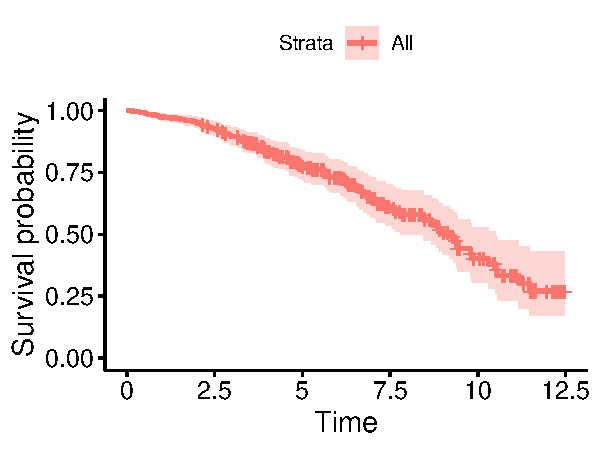
\includegraphics{report_files/figure-latex/unnamed-chunk-20-1.pdf}

A more ``manual'' approach allowed to separate a baseline survivor model
from the mean values of covariates. The reader be advised that
mentionning the ``as.factor()'' function on the edema parameter,
although already ran earlier, helped fix the plot of the baseline.

\begin{Shaded}
\begin{Highlighting}[]
\CommentTok{# Manually visualizing the estimated distribution of survival times}
\NormalTok{specimen.null<-}\KeywordTok{data.frame}\NormalTok{(}\DataTypeTok{age=}\KeywordTok{rep}\NormalTok{(}\DecValTok{0}\NormalTok{,}\DecValTok{1}\NormalTok{), }\DataTypeTok{edema=}\KeywordTok{rep}\NormalTok{(}\DecValTok{0}\NormalTok{,}\DecValTok{1}\NormalTok{), }\DataTypeTok{bili=}\KeywordTok{rep}\NormalTok{(}\DecValTok{1}\NormalTok{,}\DecValTok{1}\NormalTok{), }\DataTypeTok{albumin=}\KeywordTok{rep}\NormalTok{(}\DecValTok{1}\NormalTok{,}\DecValTok{1}\NormalTok{), }\DataTypeTok{protime=}\KeywordTok{rep}\NormalTok{(}\DecValTok{1}\NormalTok{,}\DecValTok{1}\NormalTok{), }\DataTypeTok{copper=}\KeywordTok{rep}\NormalTok{(}\DecValTok{1}\NormalTok{,}\DecValTok{1}\NormalTok{))}
\CommentTok{# for baseline}
\KeywordTok{plot}\NormalTok{(}\KeywordTok{survfit}\NormalTok{(fit.coxph, }\DataTypeTok{newdata=}\NormalTok{specimen.null), }\DataTypeTok{lwd=}\DecValTok{2}\NormalTok{,}\DataTypeTok{ylim=}\KeywordTok{c}\NormalTok{(.}\DecValTok{99}\NormalTok{,}\DecValTok{1}\NormalTok{), }\DataTypeTok{main=}\StringTok{'Baseline survivor'}\NormalTok{, }\DataTypeTok{xlab=}\StringTok{'Years'}\NormalTok{, }\DataTypeTok{ylab=}\StringTok{'Survival'}\NormalTok{, }\DataTypeTok{conf.int=}\NormalTok{T)}
\end{Highlighting}
\end{Shaded}

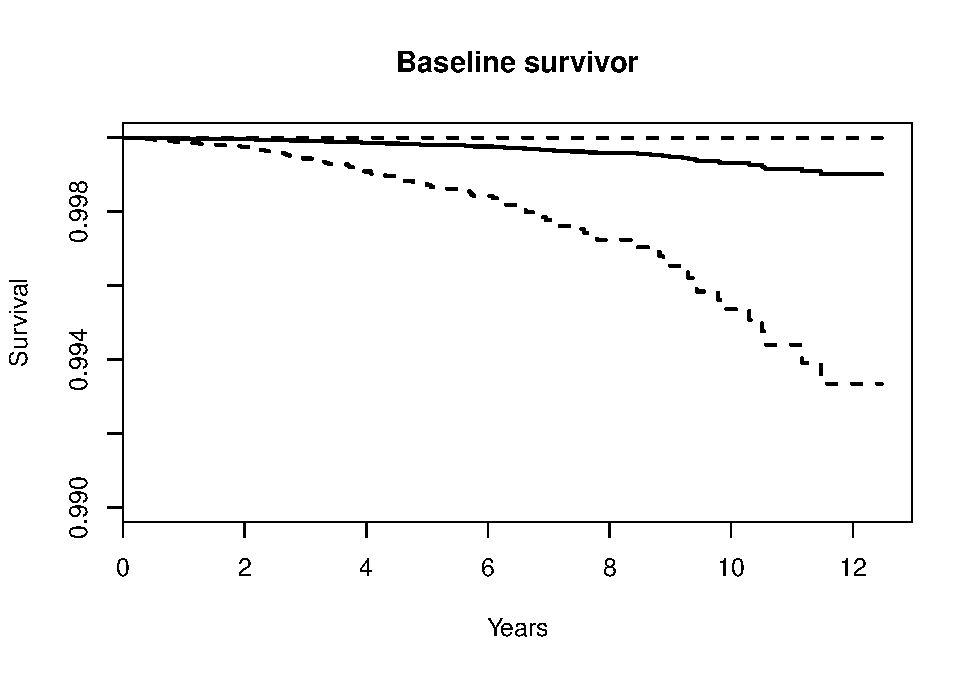
\includegraphics{report_files/figure-latex/unnamed-chunk-21-1.pdf}

\begin{Shaded}
\begin{Highlighting}[]
\CommentTok{# for mean covariates}
\KeywordTok{plot}\NormalTok{(}\KeywordTok{survfit}\NormalTok{(fit.coxph),}\DataTypeTok{lwd=}\DecValTok{2}\NormalTok{,}\DataTypeTok{main=} \StringTok{'Fitted survivor at mean covariates'}\NormalTok{, }\DataTypeTok{xlab=}\StringTok{'Years'}\NormalTok{, }\DataTypeTok{ylab=}\StringTok{'Survival'}\NormalTok{)}
\end{Highlighting}
\end{Shaded}

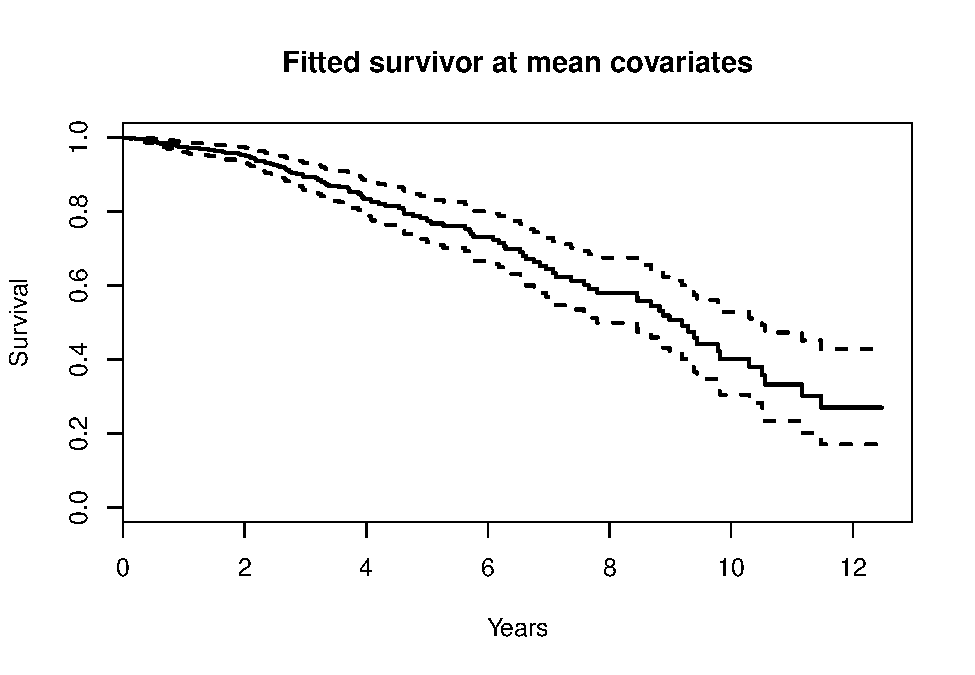
\includegraphics{report_files/figure-latex/unnamed-chunk-21-2.pdf}

Returning a unique curve for all the patients in the data set with a
confidence interval.

Various other visualizations exist such as the function ggforest() from
the survminer package which creates a forest plot for a Cox regression
model fit. Hazard ratio estimates along with confidence intervals and
p-values are plotter for each variable. One may be interested in the
forest plot for the three most significant covariates : age, bili and
albumin parameters.

\begin{Shaded}
\begin{Highlighting}[]
\KeywordTok{ggforest}\NormalTok{(}\KeywordTok{coxph}\NormalTok{(survival }\OperatorTok{~}\StringTok{ }\KeywordTok{log}\NormalTok{(bili) }\OperatorTok{+}\StringTok{ }\KeywordTok{log}\NormalTok{(albumin) }\OperatorTok{+}\StringTok{ }\NormalTok{ageBin, }\DataTypeTok{data =}\NormalTok{ specimen))}
\end{Highlighting}
\end{Shaded}

\begin{verbatim}
## Warning in .get_data(model, data = data): The `data` argument is not
## provided. Data will be extracted from model fit.
\end{verbatim}

\begin{verbatim}
## Warning: Removed 1 rows containing missing values (geom_errorbar).
\end{verbatim}

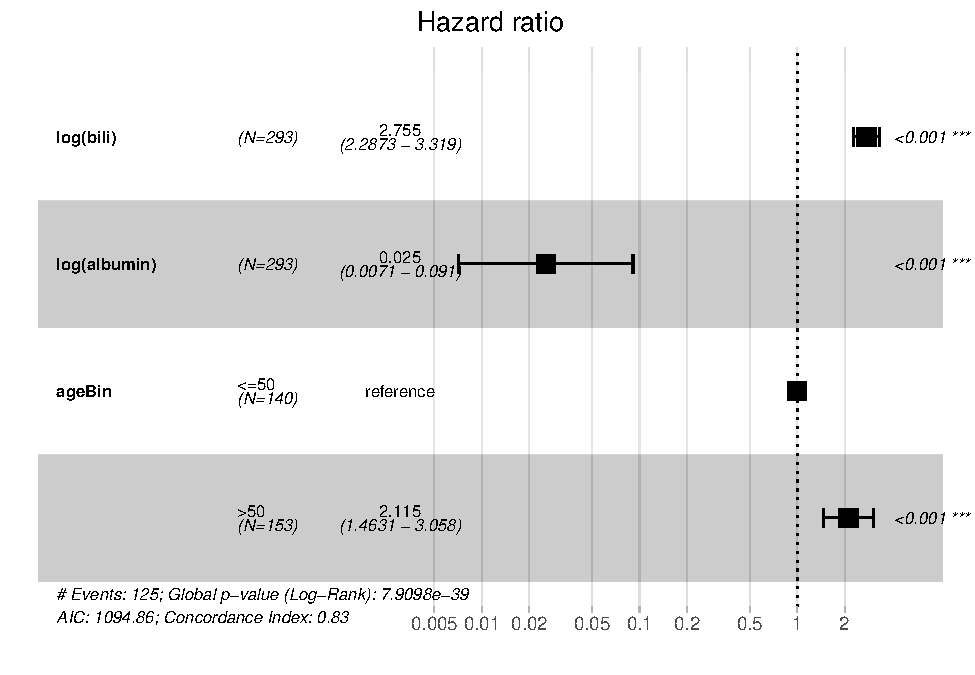
\includegraphics{report_files/figure-latex/unnamed-chunk-22-1.pdf}

From the output above one can state that the forest plot provided an
alternative view concurring the earlier stated conclusions about the
most significant covariates. The value 1 being the point at which the
covariate has no impact on the survival, the reader clearly sees that
the selected coviates do have a statistically significant impact ie. a
positive one on the left side of the 1 value and conversely a negative
one on the right side. The reader be advised of the scale especially
when interpreting the confidence intervals.

Both the isolated and joint impacts of the covariates having been
assessed through Cox Model regressions, it is of scientific requirement
and one should be now dedicated to the assurance that the Cox Model can
be applicated to the studied data set.

\subsection{Diagnostic of Cox Model}\label{diagnostic-of-cox-model}

The function cox.zph() from survival package may be used to test the
proportional hazards assumption for a Cox regression model fit. The
graphical verification of this assumption may be performed with the
function ggcoxzph() from the survminer package. For each covariate it
produces plots with scaled Schoenfeld residuals against the time.

\begin{Shaded}
\begin{Highlighting}[]
\NormalTok{ftest <-}\StringTok{ }\KeywordTok{cox.zph}\NormalTok{(fit.coxph)}
\KeywordTok{ggcoxzph}\NormalTok{(ftest)}
\end{Highlighting}
\end{Shaded}

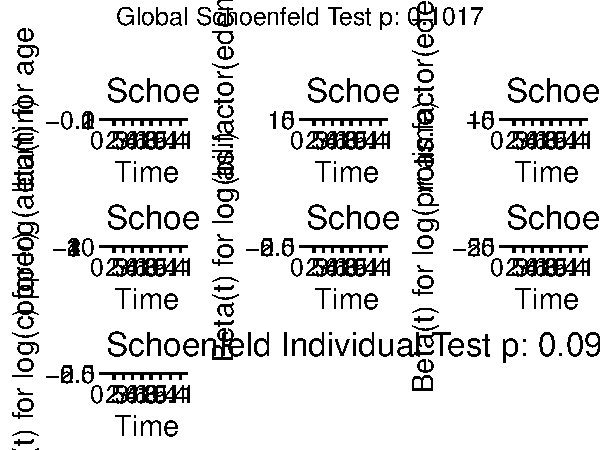
\includegraphics{report_files/figure-latex/unnamed-chunk-23-1.pdf}

The Schoenfeld Residuals Test is used to test the independence between
residuals and time and hence is used to test the proportional Hazard
assumption in Cox Model. It is analogous to testing whether the slope of
scaled residuals on time is zero or not. If the slope is not zero then
the proportional hazard assumption has been violated.

Consequently a first observation we are expecting to a flat resulting
curve in order to consider that the hazard ratio hypothesis (or
instantaneous proportional risks hypothesis) is verified. Which happens
to be the case for our selected covariates overall. And thus the Cox
regression model was validated.

Additionally the function ggcoxdiagnostics() plots different types of
residuals. The reader may be especially interested in the diagnostics of
``deviance'' for its clarity as providing an overall diagniostic by
returning a unique plot for all selected covariates.

\begin{Shaded}
\begin{Highlighting}[]
\CommentTok{# deviance vs. time}
\KeywordTok{ggcoxdiagnostics}\NormalTok{(fit.coxph,}
                 \DataTypeTok{type =} \StringTok{"deviance"}\NormalTok{,}
                 \DataTypeTok{ox.scale =} \StringTok{"time"}\NormalTok{)}
\end{Highlighting}
\end{Shaded}

\begin{verbatim}
## Warning in ggcoxdiagnostics(fit.coxph, type = "deviance", ox.scale =
## "time"): ox.scale='time' works only with type=schoenfeld/scaledsch
\end{verbatim}

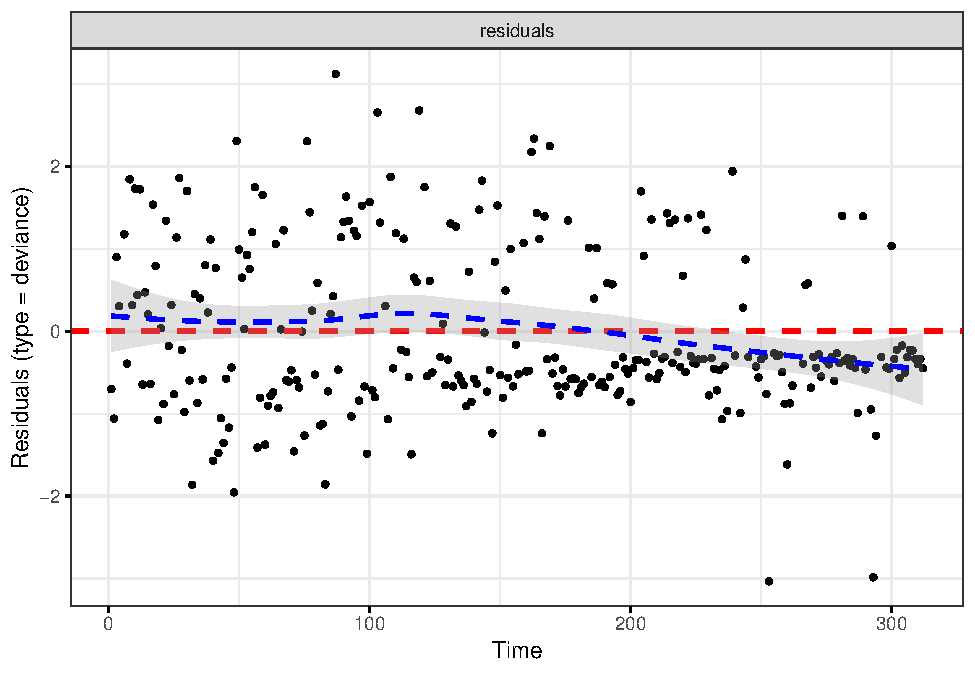
\includegraphics{report_files/figure-latex/unnamed-chunk-24-1.pdf}

Similarly the returning curve (in blue) was expected to be as flat as
possible, distributed around 0 and the data to be homogeneously
distributed on the graph in order to consider the hazard ratio
hypothesis to validate the applied Cox model on the studied data set.
Which once again appeared to be the case overall.

\section{Conclusion}\label{conclusion}


\end{document}
